\documentclass[%
	%twocolumn,
	pdftex,%              PDFTex verwenden da wir ausschliesslich ein PDF erzeugen.
	a4paper,%             Wir verwenden A4 Papier.
	landscape,%						Seite - Landscape
	ngerman,
	oneside,%             Einseitiger Druck.
	6pt,%                 Grosse Schrift, besser geeignet f�r A4.
	halfparskip,%         Halbe Zeile Abstand zwischen Abs�tzen.
]{scrbook}



\usepackage[utf8]{inputenc}

\usepackage{amssymb}
\usepackage{amsfonts}
\usepackage{verbatim}
\newcommand{\changefont}[3]{
\fontfamily{#1} \fontseries{#2} \fontshape{#3} \selectfont}

\usepackage[none]{hyphenat}
\sloppy

\usepackage{graphicx}

\usepackage[ngerman]{babel}
%\usepackage{a4wide}
\usepackage{multicol}
%\usepackage{epsfig}
% um eps-einzubinden
\usepackage[landscape]{geometry}

\usepackage{array}

\usepackage[fleqn]{amsmath}
%\usepackage{marvosym}
%\uspackage{amsopn}

\usepackage{color}
\usepackage{tabularx}

\usepackage{fancyvrb} %\usepackage{fancybox}

\usepackage{lmodern}

\usepackage{framed}

\usepackage{listings}             % Include the listings-package

\definecolor{mygreen}{rgb}{0,0.6,0}
\definecolor{mymauve}{rgb}{0.58,0,0.82}
\definecolor{lightgrey}{gray}{0.6}


\lstset{ %
  backgroundcolor=\color{white},   % choose the background 
  basicstyle=\linespread{0.9}\scriptsize,
  language=Java,
  keywordstyle=\color{blue},       % keyword style
  commentstyle=\color{mygreen},       % keyword style
  stringstyle=\color{mymauve},
  frame=single,
  framerule=1px,
  rulecolor=\color{spec_gray}, 
  aboveskip=\smallskipamount, 
  belowskip=\smallskipamount,       % 
  tabsize=1,	                   % sets default tabsize to 2 
}

%\usepackage[retainorgcmds]{IEEEtrantools} %IEEEeqnarray

\usepackage{xfrac} %f"ur sch"one 1/2 etc. Br"uche: \sfrac{1}{2}
\usepackage{cancel} %Durchstreichen in amsmath: \cance{x} oder \cancelto{0}{x}
\usepackage{enumitem}

\definecolor{spec_gray}{gray}{0.5}
\definecolor{spec_lgray}{gray}{0.65}
\definecolor{spec_blue}{rgb}{0,0.37,1}
\definecolor{spec_red}{rgb}{1,0.1,0.1}
\definecolor{spec_llgray}{gray}{0.9}

\newenvironment{bspbox}{%
  \def\FrameCommand{\fboxrule 1pt \colorbox{spec_llgray}}%
  \MakeFramed {\advance\hsize-\width \FrameRestore}}%
 {\endMakeFramed} 
 
% cp850 fr DOS, ansinew fr Windows statt latin1
%\renewcommand{\familydefault}{phv}
% setzt Helvetica (sieht aus wie Arial und sieht auch nach dvi2pdf noch gut aus)

\newcommand{\bsp}[1]{\vspace{-1.5mm}\begin{bspbox}\textbf{Bsp.:}  #1\end{bspbox}\vspace{-1mm}}

\newenvironment{mainbox}{%
  \def\FrameCommand{\fboxrule 1px \fcolorbox{black}{spec_blue}}%
  \MakeFramed {\advance\hsize-\width \FrameRestore}}%
 {\endMakeFramed}
 
\newenvironment{subbox}{%
  \def\FrameCommand{\fboxrule 1px \fcolorbox{black}{spec_gray}}%
  \MakeFramed {\advance\hsize-\width \FrameRestore}}%
 {\endMakeFramed}

\newenvironment{subsubbox}{%
  \def\FrameCommand{\fboxrule 1px \fcolorbox{black}{spec_lgray}}%
  \MakeFramed {\advance\hsize-\width \FrameRestore}}%
 {\endMakeFramed}
 
\newenvironment{titlebox}{%
  \def\FrameCommand{\fboxrule 1pt \fcolorbox{black}{black}}%
  \MakeFramed {\advance\hsize-\width \FrameRestore}}%
 {\endMakeFramed} 
 
% cp850 fr DOS, ansinew fr Windows statt latin1
%\renewcommand{\familydefault}{phv}
% setzt Helvetica (sieht aus wie Arial und sieht auch nach dvi2pdf noch gut aus)

\newcommand{\maintopic}[1]{\setcounter{subtopicenum}{0}\setcounter{subsubtopicenum}{0}\vspace{-4px}\begin{mainbox}\textcolor{white}{\textbf{\large{\stepcounter{maintopicenum}\Roman{maintopicenum}. #1}}}\end{mainbox}\vspace{-4px}}

\newcommand{\subtopic}[1]{\setcounter{subsubtopicenum}{0}\vspace{-4px}\begin{subbox}\textcolor{white}{\textbf{\stepcounter{subtopicenum}\Roman{maintopicenum}.\arabic{subtopicenum} #1}}\end{subbox}\vspace{-4px}}

\newcommand{\subsubtopic}[1]{\vspace{-3px}\begin{subsubbox}\textcolor{white}{\textbf{\stepcounter{subsubtopicenum}\Roman{maintopicenum}.\arabic{subtopicenum}.\arabic{subsubtopicenum} #1}}\end{subsubbox}\vspace{-3px}}

\newcommand{\titletopic}[1]{\vspace{0px}\begin{titlebox}\textcolor{red}{\textbf{#1}}\end{titlebox}\vspace{-3px}}

\newcommand{\vect}[1]{\mathbf{#1}}
\newcommand{\arcsinh}{\operatorname{arcsinh}}
\newcommand{\arccosh}{\operatorname{arccosh}}
\newcommand{\artanh}{\operatorname{artanh}}
\newcommand{\grad}{\operatorname{grad}}
\newcommand{\divergenz}{\operatorname{div}}
\newcommand{\rot}{\operatorname{rot}}
\newcommand{\D}{\,\textrm{d}}
\newcommand{\spec}{\operatorname{spec}}

\renewcommand\arraystretch{1.5}



\CustomVerbatimEnvironment{myverbatim}{Verbatim}{fontsize=\footnotesize,baselinestretch=0.8,numbers=none,showspaces=false,frame=single,rulecolor=\color{spec_gray}}     

\newenvironment{tight-itemize}
{ \begin{itemize}[leftmargin=*, nosep]
    \setlength{\itemsep}{0px}
    \setlength{\parskip}{0px}
    \setlength{\parsep}{0px}  }
{ \end{itemize}                  } 

\oddsidemargin-2.2cm
\evensidemargin-2.2cm
\textwidth29cm
\headheight0cm
\topmargin-2.8cm
\textheight20cm
\parskip0cm
\parindent0cm

\parskip-0.5mm


\pagestyle{empty}
%\pagenumbering{arabic}

\begin{document}\changefont{cmss}{m}{n}

\newcounter{maintopicenum}
\newcounter{subtopicenum}
\newcounter{subsubtopicenum}


\begin{multicols}{4}[][-5pt]

\setlength{\abovedisplayshortskip}{-0px}
\setlength{\abovedisplayskip}{-0px}
\setlength{\belowdisplayskip}{-0px} %Mathmode-Commands zum Platz sparen
\setlength{\arraycolsep}{2mm}

\setlength{\topsep}{4px} %Platz sparen bei Titeln
%\setlength{\parsep}{-20mm}

\raggedbottom %whitespace am Ende der letzten Seite statt verteilen des Inhalts auf ben"otigte Seiten



%\titletopic{ParProg ZF \qquad \today
%\\ Kiru \& Styp \\
%HSR FS15 \qquad Prof. Luc Bläser}
%\qquad \LaTeX{} Design Martin Stypinski
\maintopic{Begriffe}
\begin{tight-itemize}
	\item{\textbf{Parallelität}: Zerlegung eines Ablaufs in mehrere Teile, die gleichzeitig auf mehreren Prozessoren laufen. Ziel: Schnellere Programme}
	\item{\textbf{Nebenläufigkeit (Concurrency)}: Gleichzeitig oder verzahnt ausführbare Abläufe, die auf gemeinsame Ressourcen zugreifen. Ziel: Einfachere Programme}
	\item{\textbf{Prozess}: (Schwergewichtsprozess) Parallel laufende Programm-Instanz im System, Eigener Adressraum pro Prozess}
	\item{\textbf{Thread}: (Leichtgewichtsprozess) Parallele Ablaufsequenz innerhalb eines Programms, Teilen gleichen Adressraum im Prozess}
	\item{\textbf{Kontextwechsel Synchron:}	Warten auf Bedingung}
	\item{\textbf{Kontextwechsel Asynchron:} Nach gewisser Zeit soll der Thread den Prozessor freigeben. (Thread hat keinen Einfluss auf CPU Zuteilung)}
	\item{\textbf{Multi-Tasking Kooperativ:} Scheduler kann Thread nicht unterbrechen. Thread muss Kontextwechsel synchron initiieren.}
	\item{\textbf{Multi-Tasking Preemptiv:} Scheduler kann per Timer-Interrupt den laufenden Thread asynchron unterbrechen. (\textit{Time-Sliced Scheduling})}
	\item{\textbf{Synchronisation:} Einschränkung der Nebenläufigkeit \\ Fälle: Gegenseitiger Ausschluss, Warten auf Bedingungen}
\end{tight-itemize}
%\begin{center} %
%	\includegraphics[width=0.15\textwidth]{img/thread_model.png}
%\end{center}
\maintopic{Thread}
\begin{lstlisting}
public class First implements Runnable{
  @Override public void run(){}
}
public class Second extends Thread{
  @Override public void run(){}
}
public static void main(int implicitFinal,
	final int explicitFinal){
  new Thread(new First()).start();
  new Second().start(); /* new Second().run() would not
  start a new Thread (sequential) */
  new Thread(() -> { int b = implicitFinal}).start();
  new Thread(new Runnable(){
  @Override public void run(){ int a = explicitFinal; }
  }).start();
}
public void threadMethods(){
  try {
	  Thread.sleep(10); // Running -> wait 10ms -> Ready
	  Thread.yield(); // free CPU (not needed: OS preemptive)

	  Thread t = new Second();
	  t.start(); // asynchron
	  t.interrupt(); /* interrupt from outside, if Kooperative
	  Canceling (dirty) */
	  t.join(); // waits until t terminates
	  boolean isFalse = t.isAlive(); //thread is dead now

	  Thread current = Thread.currentThread(); // running Thread
	  current.setDeamon(boolean on) // Deamon Thread
  } catch (InterruptedException e) {}
}
\end{lstlisting}
\maintopic{Gefahren der Nebenläufigkeit}
\begin{tight-itemize}
	\item{\textbf{Race Condition:} Ungenügend synchronisierte Zugriffe mehrerer Threads auf gemeinsame Ressourcen (Mögliche falsche Resultate oder Verhalten)}
	\item{\textbf{Data Race: } Unsynchronisierter Zugriff auf gleichen Speicher (mind. 1 Schreibzugriff), lässt sich durch Code-Analyse systematisch finden}
	\item{\textbf{Starvation:} Kontinuierliche Fortschrittsbehinderung von Threads wegen Fairness-Problemen}
	\item{\textbf{Starvation Vermeidung:} Länger wartende Threads bevorzugen}
	\item{\textbf{Priority Inversion:} Hoch prioritärer Thread wartet auf Bedingung von tief prioritärem Thread}
	\item{\textbf{Critical Section:} Nur von einem Thread zur gleichen Zeit ausführbar}
	\item{\textbf{Mutual Exclusion:} Gegenseitiger Ausschluss (in Ciritical Section) \\
	Auf Synchronisation verzichtbare Fälle:}
	\begin{tight-itemize}
		\item{\textbf{Immutability}: Unveränderliche Objekte mit NUR lesendem Zugriff}
		\item{\textbf{Confinement}: Objekt gehört nur einem Thread zu einer Zeit.}
	\end{tight-itemize}
	\item{\textbf{Thread Confinement}: Objekt nur über Referenz von einem Thread erreichbar}
	\item{\textbf{Object Confinement}: Objekt in anderem bereits synchronisierten Objekt eingekapselt}
	\item{\textbf{Deadlock:} Gegenseitiges Aussperren (blockieren) von Threads}
	\item{\textbf{Livelock:} Deadlock, in dem Threads aber noch Instruktionen ausführen.}
	\item{\textbf{Deadlock Voraussetzungen:} Geschachtelte Locks, Zyklische Warteabhängigkeiten, Gegenseitiger Ausschluss, Sperren ohne Timeout}
	\item{\textbf{Deadlock Vermeidung:} Lineare Ordnung der Ressourcen einführen (nur geschachtelt in aufsteigender Reihenfolge sperren), grobgranulare Locks.}
	\item{\textbf{Parallele Korrektheit:} Ohne Deadlocks, Race Conditions, Starvation}
	\item{\textbf{Overrun issue:} if $\rightarrow$ while. Falls aufgeweckt, kann anderer Thread in der Zwischenzeit ändern.}
	\item{\textbf{Spurious Wakeup:} fälschliches Aufwecken in vereinzelten OS}
\end{tight-itemize}

\maintopic{Synchronisationsprimitiven - Shared Resources}
\subtopic{Monitor = synchronized}
\begin{lstlisting}
class BoundedBuffer<T> {
    private Queue<T> queue = new LinkedList<>();
    int limit; // initialize in constructor

    public synchronized void put(T x) throws InterruptedException {
        while (queue.size() == limit) {
            wait(); // await non-full
        }
        queue.add(x);
        notifyAll(); // signal non-empty
    }
    public synchronized T get() throws InterruptedException {
        while (queue.size() == 0) { // check after each waking
            wait(); // await non-empty
        }
        T x = queue.remove();
        notifyAll(); // signal non-full
        return x;
    }
    /* Nur ein Thread kann eine der synchronized Methoden in
    derselben Instanz zur gleichen Zeit ausfuehren. */
}

class Syntax {
    public static void synchronized classLock(){ }
    public        void synchronized objectLock() {}     
    public void synchronized sameSyntax(){
      synchronized(this){ } // this = monitorObject, objectLock
      synchronized(Syntax.class){} // class lock
      nestedLock(); // works because I have the lock
    }
    public void synchronized nestedLock(){
       try{
       Thread.sleep(1); // gibt lock nicht frei
       Thread.yield(); // gibt lock nicht frei
       wait(); // gibt alle gehaltenen Locks frei
       notifyAll(); // weckt alle im Monitor wartenden Threads
       notify(); // weckt einen beliebigen wartenden Thread
       }catch(InterrupedException e){
          // for spurious wakeup or Thread.interrupt();
       }
    }
}//Lockfreigabe: Blockende,Return Statement,Unhandled Exception
\end{lstlisting}
\textbf{wait(), notify() und notifyAll() nur in synchronized Block verwendbar!}

\subtopic{Semaphore}
Sehr mächtig (beliebige Synchronisation implementierbar), aber low-level
\begin{lstlisting}
class BoundedBuffer<T> {
    private Queue<T> queue = new LinkedList<>();
    private Semaphore upperLimit = new Semaphore(Capacity, true);
    private Semaphore lowerLimit = new Semaphore(0, true);
    private Semaphore mutex = new Semaphore(1, true);
    public void put(T item) throws InterruptedException {
        upperLimit.acquire(); // Warten, falls Zaehler <= 0
        mutex.acquire(); queue.add(item); mutex.release();
        lowerLimit.release();
    }
    public T get() throws InterruptedException {
        lowerLimit.acquire();
        mutex.acquire(); T item = queue.remove(); mutex.release();
        upperLimit.release();
        return item;
    }
    
    public void otherMethods(){
    // acquire(int permits) wartet, solange Zaehler < permits
    // release(int permits) Zaehler += permits
    }
}
\end{lstlisting}
\subtopic{Lock \& Conditions}
Monitor mit mehreren Wartelisten für verschiedene Bedingungen
\begin{lstlisting}
class BoundedBuffer<T> {
    private Queue<T> queue = new LinkedList<>();
    private Lock monitor = new ReentrantLock(true);
    private Condition nonFull = monitor.newCondition();
    private Condition nonEmpty = monitor.newCondition();
    public void put(T item) throws InterruptedException {
        monitor.lock();
        try {
            while (queue.size() == Capacity) { nonFull.await(); }
            queue.add(item);
            nonEmpty.signal();
        } finally { monitor.unlock(); }
    }
    public T get() throws InterruptedException {
        monitor.lock();
        try {
            while (queue.size() == 0) { nonEmpty.await(); }
            T item = queue.remove();
            nonFull.signal();
            return item;
        } finally { monitor.unlock(); }
    }
}
\end{lstlisting}
\subtopic{Read-Write Lock}
Erlaubt parallele Lese-Zugriffe
\begin{lstlisting}
ReadWriteLock rwLock = new ReentrantReadWriteLock(true);
rwLock.readLock().lock();
// read-only accesses
rwLock.readLock().unlock();
rwLock.writeLock().lock();
// write (and read) accesses
rwLock.writeLock().unlock();
\end{lstlisting}

\maintopic{Synchronisationsprimitiven - gemeinsamer Zeitpunkt}
\subtopic{CountDown Latch}
Semaphor blockiert bei $\leq$ 0, CountDown Latch bei $>$ 0,  (Latch nur fair)
\begin{lstlisting}
CountDownLatch startWhenFiveAreThere = new CountDownLatch(5);
startWhenFiveAreThere.countDown(); // Counter-1
startWhenFiveAreThere.await(); // Wait till counter == 0
// Latches sind nur einmal verwendbar.
\end{lstlisting}
\subtopic{Cyclic Barrier}
Treffpunkt für fixe Anzahl Threads, recyclierbar
\begin{lstlisting}
// Treffpunkt fuer fixe Anzahl Threads
CyclicBarrier gameRound = new CyclicBarrier(3); // 3 players
while(true){
	int parties = gameRound.getParties() //total number of players
	gameRound.await(); //returns number of missing threads
	//continues when all 3 ready, BarrierBrokenException possible!
} // gameRound.reset() - setzt CyclicBarrier zurueck
\end{lstlisting}
\subtopic{Phaser}
Verallgemeinerte Cyclic Barrier
\begin{lstlisting}
Phaser phaser = new Phaser(0); // no players at the beginning
phaser.register(); // register new players at runtime
while(...) {
  phaser.arriveAndAwaitAdvance(); // pass barrier
  playRound();
}
phaser.arriveAndDeregister();
\end{lstlisting}
\subtopic{Rendez-Vous - Exchanger}
Barriere mit Informationsaustausch
\begin{lstlisting}
Exchanger<Integer> exchanger = new Exchanger<>();
for (int k = 0; k < 2; k++) {
  new Thread(()->{
    for (int in = 0; in < 5; in++) {
      try {
        int out = exchanger.exchange(in);
        //blockiert, bis anderer Thread auch exchange() aufruft
        //und liefert Argument des jeweils anderen Threads
        System.out.println(
          Thread.currentThread().getName() + " got " + out);
      } catch (InterruptedException e) { }
    }
  }).start();
}
\end{lstlisting}
\maintopic{Thread Pool Konzept}
\begin{tight-itemize}
	\item{\textbf{Task Queue:} Tasks in Warteschlange (parallel und beliebige Reihenfolge!)}
	\item{\textbf{Thread Pool:} Beschränkte Anzahl Worker-Threads bearbeiten Tasks}
	\item{\textbf{Pool Vorteile:} Beschränkte Anzahl Threads, Recycling der Threads, Höhere Abstraktion, Anzahl Threads pro System konfigurierbar}
	\item{\textbf{Pool Einschränkungen:} Tasks müssen unabhängig sein (dürfen nicht aufeinander warten), Run to completion (Stack wieder frei machen)}
	\item{\textbf{Future:} repräsentiert ein zukünftiges Resultat eines asynchronen Calls.\\
	Bei unbehandelter Exception liefert get() eine \textit{ExecutionException} mit der ursprünglichen Exception darin geschachtelt (\textit{Cause}).}
\end{tight-itemize}

\begin{lstlisting}
ForkJoinPool threadPool = new ForkJoinPool();
List<Future<Long>> futures = new ArrayList<>();

for (int count = 1; count <= 8; count++) {
	long n = count * 100000000000000000L;
	futures.add(threadPool.submit(() -> Computation.nextPrime(n)));
} // Future<T> future = threadPool.submit();
for (Future<Long> future: futures) {
	System.out.println("Result: " + future.get());
} // T result = future.get(); wait until result is set
\end{lstlisting}
\columnbreak
\maintopic{Recursive Tasks}
\begin{lstlisting}
import java.util.concurrent.RecursiveTask;
public class CountTask extends RecursiveTask<Integer> {
	private final int lower, upper;
	
	public CountTask(int lower, int upper) {
		this.lower = lower; this.upper = upper;
	}
	protected Integer compute() {
		if (lower == upper) {return 0;}
		if (lower + 1 == upper) {return isPrime(lower) ? 1 : 0;}
		int middle = (lower + upper) / 2;
		CountTask left = new CountTask(lower, middle);
		CountTask right = new CountTask(middle, upper);
		left.fork(); right.fork(); // start as sub-task in new task
		return right.join() + left.join(); // wait until task ends
	}
}// Improvement: if (upper-lower>Threshold).. else sequential
// Call: (invoke() is submit() and future.get() in one call)
ForkJoinPool threadPool = new ForkJoinPool();
int result = threadPool.invoke(new CountTask(2, INPUT_SIZE));
\end{lstlisting}
\maintopic{Asynchrone Programmierung}
\begin{tight-itemize}
	\item{\textbf{Caller-zentrisch (Pull):} warten auf Task-Ende (Future abfragen)}
	\item{\textbf{Callee-zentrisch (Push):} Asynchrone Operation (Completion Callback)}
\end{tight-itemize}
\begin{lstlisting}
CompletableFuture<Long> future = CompletableFuture
	.supplyAsync(() -> longOperation()); // (runAsync(), if void)
// other work
process(future.get());
// or
future.thenAccept(result -> System.out.println(result)); //void
future.thenApply(f2).thenAccept(f3); // if return value needed
// Multi Continuation:
CompletableFuture.allof(f1, f2).thenAccept(continuation);
ComplteableFuture.any(f1, f2).thenAccept(continuation);
\end{lstlisting}
\maintopic{.NET Task Parallel Library (TPL)}
\begin{tight-itemize}
	\item{\textbf{Exception in Threads:} führt zu Abbruch des gesamten Programms.}
	\item{\textbf{volatile} auch von java kopiert}
	\item{\textbf{Lokale Variabeln:} Lokale Variablen müssen nicht Read-only (final) sein.}
	\item{\textbf{Delegate:} Referenz auf Methode}
	\item{Lambda kann auf umgebende Variablen zugreifen (\textbf{Data Race Gefahr})}
	\item{Pulse() informiert längst Wartenden (FIFO Warteschlange)}
\end{tight-itemize}	
\begin{lstlisting}
class BankAccount {
  private decimal balance;
  private object syncObject = new object(); // helper for this
  public void Withdraw(decimal amount) {
    lock(syncObject) { // synchronized
      while (amount > balance) { // loop with condition
        Monitor.Wait(syncObject);
      }
      balance -= amount;
    }
  }
  public void Deposit(decimal amount) {
    lock(syncObject) {
     balance += amount;
         Monitor.PulseAll(syncObject); // notifyAll()
    }
  }
}
/* --- */
Task task = Task.Run(() => {
   // task implementation
}); // only access final variables from inside!
task.Wait(); // blocks until task ends
// Task<int> + task.Result // wait for result
// Task.WaitAll(taskA, taskB); // wait for two tasks
// TPL
ThreadPool.SetMaxThreads(100);//else dynamic (Thread Injection)
long sum = 0; // Korrekte Parallele Aggregation mit Lock:
Parallel.ForEach(list, file => {
  int subTotal = ..
  lock(someLockObject){ //atomare Instruktion waere effizienter
    sum += subTotal;
  }
});
Parallel.For(0, array.Length, i => doStuff(array[i]));
Parallel.Invoke(() => FirstAction(a, b), ...); //maybe parallel
// Task Continuations
task1.WhenAll(t1, t2).WhenAny(t3, t4).ContinueWith(t5)
\end{lstlisting}
\subtopic{Async \& Await Fehler}
\begin{tight-itemize}
    \item{Versehentlicher blockierender async: await vergessen, Methode ist synchron}
    \item{Threadwechsel innerhalb der Methode: Vorsicht lokale Variablen!}
    \item{Quasiparallelität: foreach von collection -> collection kann verändert werden}
    \item{Race-condition möglich}
    \item{UI-Deadlock: return await Task.Run(..)}
\end{tight-itemize}
\newpage
\maintopic{GUI}
\begin{tight-itemize}
	\item{GUI-Frameworks erlauben nur Single-Threading (UI-Thread)}
	\item{Gründe: Synchronisationskosten (Locking), Deadlock Risiko (z.B. MVC)}
	\item{Einschränkungen: keine langen Operationen, Thread Confinement}
	\item{\textbf{Thread Confinement:} Nur UI-Thread darf auf UI Komponenten zugreifen}
	\item{Andere Threads müssen UI-Änderungen als Events an UI-Thread senden}
\end{tight-itemize}
\begin{lstlisting}
// Java (UI-Thread = Event Dispatching Thread (EDT))
SwingUtitilties.invokeLater(() -> { // clean Swing GUI setup
	frame.pack(); frame.setVisible(true);
}); //run in UI-Thread (end of main method)
SwingUtitilties.invokeAndWait(runnable); // synchronous
// .Net: call is sync
async Task<string> ConcatWebSitesAsync(string url1, string url2) {
    HttpClient client = new HttpClient();
    Task<string> download1 = client.GetStringAsync(url1);
    Task<string> download2 = client.GetStringAsync(url2);
    // now the following part is async
    string site1 = await download1; // runs in separate thread
    string site2 = await download2;
    // oder 'site1 = await new Task(() -> myMethod());
    return site1 + site2;
} //async without await: warning; await not inside async: error
// special case UI
async void startDownload_Click(...) {
    HttpClient client = new HttpClient();
    foreach (var url in collection) {
        var data = await client.GetStringAsync(url);
        textArea.Content += data;
    }//problem: collection might change --> make copy (snapshot)
}
\end{lstlisting}
\maintopic{Memory Model}
\begin{tight-itemize}
	\item{Ursachen für Probleme}
	\begin{tight-itemize}
	    \item{\textbf{Weak Consistency:} Sepeicherzugriffe in unbestimmter Reihenfolge}
	    \item{\textbf{Optimierungen:} Änderungen von Compiler, Laufzeitsystem, CPUs}
   	\end{tight-itemize}
    \item{\textbf{JVM Minimale Garantien} Atomicity (Unteilbarkeit), Visibility (Sichtbarkeit), Ordering (Reihenfolge)}
    \item{\textbf{Java Atomicity Garantien:} Zugriff auf primitive Datentypen bis 32bit und Objekt-Referenzen atomar, \textbf{volatile} Variable atomar (z.B. long/double), Instanziierung mit Zuweisung nicht atomar}
    \item{\textbf{Java Visibility garantiert bei:} Locks Release \& Acquire, Volatile Variable, Initialisierung von final Variablen (nach Ende des Konstruktors), Thread Start und Join (ebenso Task Start / Ende)}
    \item{\textbf{Java Ordering Garantien:} Innerhalb Threads As-If-Serial, Zwischen Threads Reihenfolge gleich für Synchronisationsbefehle, volatile Variablen}
    \item{\textbf{Java Volatile Keyword} Atomares schreiben für long und double, Änderungen werden anderen Zugreifenden propagiert, Kein Umordnen durch Compiler / Laufzeitsystem / CPU}
\end{tight-itemize}
\begin{lstlisting}
public class SpinLock{
  private final AtomicBoolean locked = new AtomicBoolean(false);
  public void acquire(){
    while(locked.getAndSet(true)){ Thread.yield(); }
  }
  public void release(){ locked.set(false); }
  // locked.compareAndSet(expected, update) true if successful
  // locked.updatedAndGet(x -> true);
}
// Optimistische Synchronisation (ABA Problem)
do{ // other thread may change and change back value in between
    oldValue = var.get();
    newValue = calculateChanges(oldValue);
} while(!var.compareAndSet(oldValue, newValue));
// in Java 8: var.updatedAndGet(old -> calculateChanges(old));
AtomicReference<Node<T>> top = new AtomicReference<>();
// Lock-Free Stack
void push(T value) {
  Node<T> newNode = new Node<>(value);
  Node<T> current;
  do {
    current = top.get();
    newNode.setNext(current);
  } while (!top.compareAndSet(current, newNode));
}
\end{lstlisting}
\begin{center}
    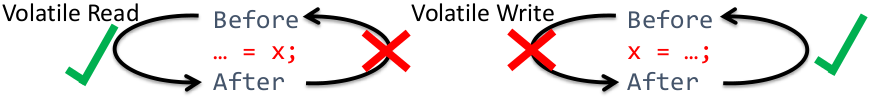
\includegraphics[width=0.2\textwidth]{img/volatile.png}
\end{center}
Unterschiede .NET: long/double nicht mit volatile atomar, visibility nicht definiert, Ordering: volatile nur partial fence (Thread.MemoryBarrier();)
\maintopic{Actor}
\begin{tight-itemize}
	\item{\textbf{Vorteile:} Aktive Objekte, kein Shared Memory, Kommunikation zwischen Objekten, keine Data Races mehr (Race Conditions schon noch), Distributed Concurrency möglich}
\end{tight-itemize}
\begin{lstlisting}
public class NumberPrinter extends UntypedActor { // Akka Actor
 public void onReceive(final Object message) {
  if (message instanceof Integer) {//communicates with messages
    System.out.print(message);
  } // onReceive(): "Run to Completion" per received message
 }
}
ActorSystem system = ActorSystem.create("System")
ActorRef printer = system.actorOf(Props.create(NumberPrinter.class));
for (int i = 0; i < 100; i++) {
    printer.tell(i, ActorRef.noSender());//tell(message, sender)
}
Future<Object> result = Patterns.ask(actorRef, msg, timeout);
system.shutdown(); // give end-signal to all actors
\end{lstlisting}
Wieso \textbf{ActorRef}: Adresse eines Actors (bei Fehlverhalten neu startbar), Entkopplung von Interface und Instanz, immutable (verschickbar)
\maintopic{GPU Parallelisierung}
\begin{tight-itemize}
	\item{GPUs bieten mehr Cores, sind dafür sehr spezifisch und langsamer}
	\item{\textbf{Streaming Multiprocessor} (SM) hat mehrere \textbf{Streaming Processor} (SP)}
  	\item{\textbf{SIMD}: Single Instruction Multiple Data, Vektorparalleliserung}
    \item{\textbf{NUMA}: Non-Uniform Memory Access: Host-Memory zu Device-Memory}
    \item{\textbf{CUDA Block}: Threads sind in Blöcke gruppiert (1 Block $\rightarrow$ gleicher SM)}
    \item{\textbf{Grid}: Hat mehrere Blöcke}
    \item{\textbf{Thread} = virtueller Skalarprozessor}
    \item{\textbf{Block} = virtueller Multiprozessor (Blöcke müssen unabhängig sein, run-to-completion, Grösse: vielfaches von 32)}
    \item{\textbf{Shared Memory}: Per SM, schnell (4 Zyklen), nur zwischen Threads innerhalb Block sichtbar, ein paar KB $\rightarrow$ \lstinline|__shared__ float x;|}
    \item{\textbf{Global Memory}: Main Memory, langsam (400-600 Zyklen), allen Threads sichtbar, mehrere GB $\rightarrow$ \lstinline|cudaMalloc();|}
    \item{\textbf{Warp}: Block wird intern in Warps zerlegt (zu 32-Threads)}
    \item{Block läuft auf SM, Warp läuft (falls aktiv) auf SPs eines einzigen SM}
    \item{\textbf{Divergenz}: Unterschiedliche Verzweigung im selben Warp: SM führt abwechselnd Instruktionen der Verzweigungen durch, die anderen warten}
    \item{\textbf{Memory Coalescing}: Zugriffsmuster der Threads sind entscheidend, falls aufeinanderfolgende Daten $\rightarrow$ in einer Transaktion (\textbf{Memory Burst})}
    \item{\textbf{Launch Configuration} (Grid/Block Dimensionierung): Maximale Anzahl Threads pro Block, Blockgrösse vielfaches von 32, wenig unnütze Threads}
    \item{\textbf{$\rightarrow$ Performance-Aspekte}: Shared Memory, GPU Utilization, Divergenz}
\end{tight-itemize}

\begin{lstlisting}
void CudaVectorAdd(float* A, float* B, float* C, int N) {
  size_t size = N * sizeof(float);
  float *d_A, *d_B, *d_C;
  // in Device Memory (GPU) allozieren
  handle(cudaMalloc(&d_A, size)); 
  handle(cudaMalloc(&d_B, size));
  handle(cudaMalloc(&d_C, size));
  // Daten zu GPU transferieren
  handle(cudaMemcpy(d_A, A, size, cudaMemcpyHostToDevice));
  handle(cudaMemcpy(d_B, B, size, cudaMemcpyHostToDevice));
  
  int blockDim = 512, gridDim = (N + blockDim - 1) / blockDim;
  //gridDim = Anzahl Bloecke, blockDim Anzahl Threads per Block
  VectorAddKernel<<<gridDim, blockDim>>>(d_A, d_B, d_C, N);
  handle(cudaGetLastError()); // da vorherige Rueckgabe void
  // Daten von GPU zurueck zu CPU transferieren
  handle(cudaMemcpy(C, d_C, size, cudaMemcpyDeviceToHost));
  // in Device Memory (GPU) deallozieren
  handle(cudaFree(d_A)); handle(cudaFree(d_B));
  handle(cudaFree(d_C));
}
void handle(cudaError error) {
  if (error != cudaSuccess) {
    fprintf(stderr, "CUDA: %s!\n",
    cudaGetErrorString(error));
    exit(EXIT_FAILURE);
  }
}
__global__ // kernel definition
void VectorAddKernel(float *A, float *B, float *C, int N) {
  int i = blockIdx.x * blockDim.x + threadIdx.x; // Aufteilung
  if (i < N) {    C[i] = A[i] + B[i];   }
}/* if: Boundary Check, falls aufgerundet wurde -> mehr Threads
als zu bearbeitende Daten */
// 3D Blocks / Grid
dim3 gridDim(3, 2, 1); dim3 blockDim(4,3,1);
Function<<gridDim, blockDim>>();
// Jagged array (in C nicht direkt unterstuetzt)
float *matrix =
(float *)malloc(NofRows * NofCols * sizeof(float));
matrix[row * NofCols + col] = //..
// Matrix Multiplikation
__global__
void multiply(float *A, float *B, float *C) {
  int i = blockIdx.x * blockDim.x + threadIdx.x;
  int j = blockIdx.y * blockDim.y + threadIdx.y;
  if (i < N && j < M) { // Randbehandlung
    float sum = 0;
    for (int k = 0; k < K; k++) {
      // sum += A[i,k ] * B[k,j]
      sum += A[i * K + k] * B[k * M + j];
    }
    C[i * M + j] = sum; // C[i,j] = sum
  }
}
// Matrix Multiplikation mit Shared Memory
__shared__ float Asub[TILE_SIZE][TILE_SIZE];
__shared__ float Bsub[TILE_SIZE][TILE_SIZE];

int tx = threadIdx.x, ty = threadIdx.y;
int col = blockIdx.x * TILE_SIZE + tx;
int row = blockIdx.y * TILE_SIZE + ty;

for (int tile = 0; tile < nofTiles; tile++) {
  Asub[ty][tx] = A[row * K + tile * TILE_SIZE + tx];
  Bsub[ty][tx] = B[(tile * TILE_SIZE + ty) * M + col];
  __syncThreads(); // wartet auf alle Threds innerhalb Block
  for (int ksub = 0; ksub < TILE_SIZE; ksub++) {
    sum += Asub[ty][ksub] * Bsub[ksub][tx];
  }
  __syncThreads(); // 2. Barriere
}
C[row * M + col] = sum;
// Divergenz: gut, da gleiche Verzweigung innerhalb eines Warps
if (threadIdx.x / 32 > 1) { } else { }
// Coalescing ist gut falls + threadIdx.x
data[(Ausdruck ohne threadIdx.x) + threadIdx.x]
\end{lstlisting}
\maintopic{Cluster und High-Performance Computing (HPC)}
\begin{tight-itemize}
	\item{\textbf{Head Node}: Zugriffspunkt (restliche sind \textbf{Compute Nodes})}
	\item{Job Manager für Monitoring}
	\item{\textbf{HPC Job}: vom Client lanciert, besteht aus mehreren Tasks}
	\item{\textbf{HPC Task}: Ausführung eines Executables, Operiert auf Files in File Share, Abhängigkeiten zwischen Tasks definierbar}
	\item{Schwierigkeiten verteilter Ausführung: kein Shared Memory $\rightarrow$ Messages} 
	\item{\textbf{MPI}: basiert auf Actor/CSP, Standard für heterogene Parallelisierung}
	\item{Communicator: Gruppen von MPI Prozessen (erlaubt Kommunikation)}
	\item{Communicator World: Alle Prozesse einer Ausführung (eigene Gruppen)}
\end{tight-itemize}

\begin{lstlisting}
// start: mpiexec -n 16 FirstMpiProgram.exe
var world = Communicator.world;
world.Rank // Process-ID (0..Size-1)
world.Size // Total number of processes
world.Send(value, receiverRank, messageTag); // send msg
world.Receive(senderRank, messageTag, out value);//receive msg
world.Broadcast(ref value, senderRank); // send msg to all
world.Barrier() // wait for all processes
var request = world.ImmediateSend(val, recRank, msgTag);//async
// -> request.Wait(); // future
// Teilresultate aggregieren, jeder erhaelt Gesamtresultat
world.Allreduce(value, (a,b) => a + b); // broadcast
// Nur ein Prozess (rank) sieht Gesamtresultat (effizienter)
world.Reduce(value, (a,b) => a + b, rank);
// jeder sendet verschiedenen Wert an alle anderen
// nachher haben alle die Werten von jedem
outputArray = Alltoall(inputArray);
// einer verteilt verschiedene Werte an alle anderen
value = Scatter(array, senderRank);
// alle senden verschiedenen Wert an einen
outputArray = Gather(value, receiverRank);
\end{lstlisting}

\maintopic{Reactive Programming (Rx = Reactive Extensions)}
\begin{tight-itemize}
	\item{PLINQ: Resultate ungeordnet (bei Java 8 Streams geordnet)}
	\item{Pull (LINQ): Pipeline-Steps rückwärts, Input-Quelle passiv und \textbf{komplett}}
	\item{Push (Reactive): Input/Arbeitsschritt aktiv, pro Wert ein Event (OnNext)}
	\item{Rx: Subject (Promise) = Observable + Observer}
\end{tight-itemize}

\begin{lstlisting}
var subject = new Subject<string>();
subject.Subscribe(Console.WriteLine);
subject.OnNext("A");
subject.OnCompleted(); // successful end of sequence
subject.OnError() // end if error
subject.Subscribe(delegateNext, delegateError, delegateComplete);

// Subject: keine alten Werte, kein buffer
// ReplaySubject: alle alte Werte, unlimited Buffer
// BehaviorSubject: observer hat letzten Wert, 1 Element Buffer
// AsyncSubject: letzter Wert bei OnComplete, 1 Element Buffer
var replay = new ReplaySubject<string>();

var merged = oneEnumerable.ToObservable().Merge(secondSubject);
// default sequential + async
subject.ObserverOn(TaskPoolScheduler.Default); // set parallel
subject.ObserveOnDispatcher().Subscribe(); // in UI-Thread
// Possible Race Condition (side effects in observer)
// Possible Deadlock (dependency in Observer: First(), Last())
// hot = aktiv: notifizieren spontan, ohne registrierte Observer
// cold = passiv: notifizieren on request, erst bei Anmeldung
\end{lstlisting}

\maintopic{Software Transactional Memory}
\begin{tight-itemize}
    \item{Atomare Operations-Sequenzen, keine inkonsistenten Zwischenzustände}
    \item{ACI TX: Atomicity (vollständig oder gar nicht sichtbar), Consistency (Programm vor und nach Transaktion gültig), Isolation (as-if-serial)}
    \item{Gegensatz zu DB: Keine Durability / Persistenz}
    \item{Deskriptive Programmierung, automatische Isolation (nur Speicher- Zugriffe, Seiteneffekte nicht), meist Optimistic Concurrency control OCC}
    \item{Probleme: Starvation (OCC), Seiteneffekte in SW-TX bleiben sichtbar}
    \item{Einschränkung: kein I/O, nur Lesen von final und lokalen Variablen}
    \item{Scala: Write Skew nicht möglich, Starvation problem}
\end{tight-itemize}

\begin{lstlisting}
final Ref.View<Integer> balance = STM.newRef(0); //var wrapping
void deposit(int amount) { // type T must be immutable!
  STM.atomic(() -> {
    balance.set(balance.get() + amount);
  });
}
void withdraw(int amount) {
  STM.atomic(() -> {
    if (balance.get() < amount) {
      STM.retry(); // Abbruch und automatische Wiederholung
    }
    balance.set(balance.get() - amount);
  });
} // bei Exception -> Rollback und Abbruch
// write sekew:
atomic { if (b.onDuty) { a.onDuty = false; } }
atomic { if (a.onDuty) { b.onDuty = false; } }
\end{lstlisting}

\maintopic{Misc}
\begin{lstlisting}
Collections.synchronizedList(list); 
/ ..Collection(...) / ..Map...()
// Lockfreie Datenstrukturen
ConcurrentLinkedQueue<V>, ConcurrentLinkedDeque<V>
ConcurrentSkipListSet<V>, ConcurrentHashMap<K, V>
ConcurrentSkipListMap<K, V>
\end{lstlisting}

\begin{tight-itemize}
    \item{OutOfMemory Gründe: Kosten zwischen 128kB bis 1MB pro Thread}
    \item{notifyAll()?: Notify() genügt, wenn alle auf eine Bedingung warten.}
\end{tight-itemize}

\begin{lstlisting}
public class UpgradeableReadWriteLock {
  private ReadWriteLock readWriteLock = 
  new ReentrantReadWriteLock(true);
  private Lock mutex = new ReentrantLock(true);

  public void readLock() throws InterruptedException {
    readWriteLock.readLock().lock();
  }
  public void readUnlock() {
    readWriteLock.readLock().unlock();
  }
  public void upgradeableReadLock() throws InterruptedException {
    mutex.lock();
  }
  public void upgradeableReadUnlock() { mutex.unlock(); }
  public void writeLock() throws InterruptedException {
    mutex.lock(); readWriteLock.writeLock().lock();
  }
  public void writeUnlock() {
    mutex.unlock(); readWriteLock.writeLock().unlock();
  }
}
//--
CompletableFuture<String> as =
    CompletableFuture.supplyAsync(() -> { });
as.thenAccept(result -> {});
// ForkJoinPool
invokeAll(a, b) == a.fork(); b.fork(); b.join(); a.join();
// --
// lock free stack - herausnehmen, falls platzmangel
public class LockFreeStack<T> implements Stack<T> {
  private AtomicReference<StackNode<T>> topNode;
  private StackNode<T> bottomElement = new StackNode<T>(null);
  public LockFreeStack(){
    topNode = new AtomicReference<>(bottomElement);
  }
  public void push(T value) {
    StackNode<T> curTop;
    StackNode<T> nextTop;
    do{
        curTop = topNode.get();
        nextTop = new StackNode<>(curTop, value);
    }while (!topNode.compareAndSet(curTop, nextTop));
  }
  public T pop() {
    StackNode<T> curTop;
    do{
      curTop = topNode.get();
    }while(curTop != bottomElement
    && !topNode.compareAndSet(curTop, curTop.getNextElement()));
    return curTop.getValue();
  }
}
// AtomicInteger a = new AtomicInteger(10);
// a.updateAndGet(i -> i + 2);
\end{lstlisting}

\maintopic{Checklist}
\begin{tight-itemize}
    \item{ThreadPool: Shutdown nicht vergessen}
    \item{GPU: Boundary Check wegen zusätzlichen Threads}
    \item{bei wait() / Condition.await() $\rightarrow$ InterruptedException nicht vergessen}
    \item{try-final nicht vergessen, wenn lock}
    \item{Bei CyclicBarrier.await() ist BarrierBrokenException möglich}
    \item{Spurious wakeup auch möglich als Fehler.}
    \item{Nur Getter / Setter synchronized falsch! (Critical section ist grösser)}
    \item{Exception-Handling bei \textit{Fire and Forget} nicht vergessen!}
\end{tight-itemize}
\begin{center}
	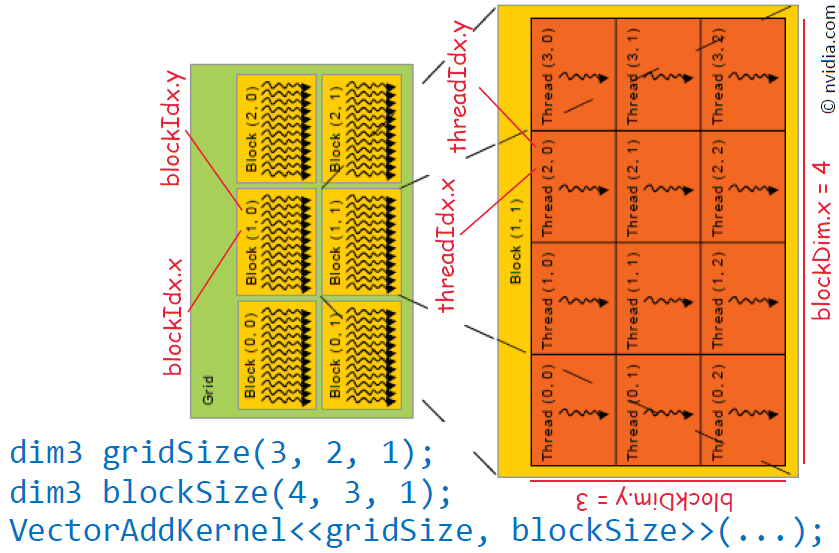
\includegraphics[width=0.17\textwidth]{img/cuda-grid-and-blocks.png}
\end{center}
\end{multicols}

\end{document}
